\documentclass{article}%
\usepackage[T1]{fontenc}%
\usepackage[utf8]{inputenc}%
\usepackage{lmodern}%
\usepackage{textcomp}%
\usepackage{lastpage}%
\usepackage{geometry}%
\geometry{tmargin=1cm,lmargin=3cm,rmargin=3cm}%
\usepackage{graphicx}%
\usepackage{amsmath}%
%
%
%
\begin{document}%
\normalsize%
\section{Introduction}%
\label{sec:Introduction}%
In this project, I implement a 3  ×  3 Hill Cipher Machine in Python. This machine automatically generates LaTeX reports to decipher user{-}entered Hill Ciphers step by step. \newline%
 \newline%
%
We will be deciphering: IQCWTM using the key: GYBNQKURP. \newline%
 \newline%
%
Note that the cipher and key in the line above have been entered by the user.

%
\section{Encryption Matrix}%
\label{sec:EncryptionMatrix}%


\begin{figure}[h!]%
\centering%
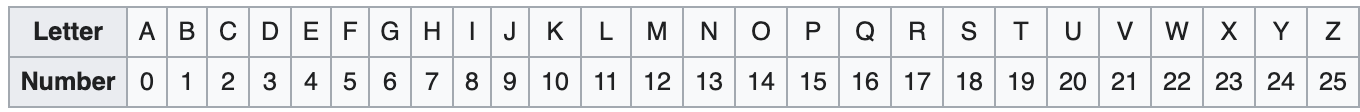
\includegraphics[width=420px]{./LookupHill.png}%
\caption{Lookup Table for Hill Cipher (Wikipedia)}%
\end{figure}

%
We use the Lookup Table above and our key GYBNQKURP to create the Encryption Matrix below: \newline%
%
\[%
\begin{pmatrix}%
6.0&24.0&1.0\\%
13.0&16.0&10.0\\%
20.0&17.0&15.0%
\end{pmatrix}%
\]

%
\section{Finding the Decryption Matrix (Encryption Matrix Inverse Mod 26)}%
\label{sec:FindingtheDecryptionMatrix(EncryptionMatrixInverseMod26)}%
We now find the modular (26) inverse of the Encryption Matrix to decrypt our message. \newline%
 \newline%
%
We first reduce our Augmented Encryption Matrix (M) to the Identity Matrix: \newline%
 \newline%
%
\[%
E21 * E31 * M:%
\]%
\[%
\begin{pmatrix}%
1.0&0.0&0.0\\%
-2.167&1.0&0.0\\%
-3.333&0.0&1.0%
\end{pmatrix} \begin{pmatrix}%
6.0&24.0&1.0&1.0&0.0&0.0\\%
13.0&16.0&10.0&0.0&1.0&0.0\\%
20.0&17.0&15.0&0.0&0.0&1.0%
\end{pmatrix} = \begin{pmatrix}%
6.0&24.0&1.0&1.0&0.0&0.0\\%
0.0&-36.0&7.83&-2.17&1.0&0.0\\%
0.0&-63.0&11.67&-3.33&0.0&1.0%
\end{pmatrix}%
\]%
\newline%
%
\[%
E32 * E21 * E31 * M:%
\]%
\[%
\begin{pmatrix}%
1.0&0.0&0.0\\%
0.0&1.0&0.0\\%
0.0&-1.75&1.0%
\end{pmatrix} \begin{pmatrix}%
6.0&24.0&1.0&1.0&0.0&0.0\\%
0.0&-36.0&7.83&-2.17&1.0&0.0\\%
0.0&-63.0&11.67&-3.33&0.0&1.0%
\end{pmatrix} = \begin{pmatrix}%
6.0&24.0&1.0&1.0&0.0&0.0\\%
0.0&-36.0&7.83&-2.17&1.0&0.0\\%
0.0&0.0&-2.04&0.46&-1.75&1.0%
\end{pmatrix}%
\]%
\newline%
%
\[%
E23 * E13 * E32 * E21 * E31 * M:%
\]%
\[%
\begin{pmatrix}%
1.0&0.0&0.49\\%
0.0&1.0&3.84\\%
0.0&0.0&1.0%
\end{pmatrix} \begin{pmatrix}%
6.0&24.0&1.0&1.0&0.0&0.0\\%
0.0&-36.0&7.83&-2.17&1.0&0.0\\%
0.0&0.0&-2.04&0.46&-1.75&1.0%
\end{pmatrix} = \begin{pmatrix}%
6.0&24.0&0.0&1.22&-0.86&0.49\\%
0.0&-36.0&0.0&-0.41&-5.71&3.84\\%
0.0&0.0&-2.04&0.46&-1.75&1.0%
\end{pmatrix}%
\]%
\newline%
%
\[%
E12 * E23 * E13 * E32 * E21 * E31 * M:%
\]%
\[%
\begin{pmatrix}%
1.0&0.67&0.0\\%
0.0&1.0&0.0\\%
0.0&0.0&1.0%
\end{pmatrix} \begin{pmatrix}%
6.0&24.0&0.0&1.22&-0.86&0.49\\%
0.0&-36.0&0.0&-0.41&-5.71&3.84\\%
0.0&0.0&-2.04&0.46&-1.75&1.0%
\end{pmatrix} = \begin{pmatrix}%
6.0&0.0&0.0&0.95&-4.67&3.05\\%
0.0&-36.0&0.0&-0.41&-5.71&3.84\\%
0.0&0.0&-2.04&0.46&-1.75&1.0%
\end{pmatrix}%
\]%
\newline%
%
\[%
D * E12 * E23 * E13 * E32 * E21 * E31 * M:%
\]%
\[%
\begin{pmatrix}%
0.17&0.0&0.0\\%
0.0&-0.03&0.0\\%
0.0&0.0&-0.49%
\end{pmatrix} \begin{pmatrix}%
6.0&0.0&0.0&0.95&-4.67&3.05\\%
0.0&-36.0&0.0&-0.41&-5.71&3.84\\%
0.0&0.0&-2.04&0.46&-1.75&1.0%
\end{pmatrix} = \begin{pmatrix}%
1.0&0.0&0.0&0.16&-0.78&0.51\\%
0.0&1.0&-0.0&0.01&0.16&-0.11\\%
0.0&0.0&1.0&-0.22&0.86&-0.49%
\end{pmatrix}%
\]%
\newline%
%
Then, in the final step, we multiply the regular inverse with its determinent. Then we multiply it with its detrminent's 'modular (26) inverse'. Then we write the whole matrix mod 26:%
\[%
25 * 441 *  \begin{pmatrix}%
0.16&-0.78&0.51\\%
0.01&0.16&-0.11\\%
-0.22&0.86&-0.49%
\end{pmatrix} = \begin{pmatrix}%
8.0&5.0&10.0\\%
21.0&8.0&21.0\\%
21.0&12.0&8.0%
\end{pmatrix} (mod  26)%
\]%
\newline%

%
\section{Matrix Multiplications}%
\label{sec:MatrixMultiplications}%
Now that we have the inverse/decryption matrix, we will multiply our cipher IQCWTM with the decryption matrix in chunks of 3. For each cipher chunk, we will create a decryption vector to multiply using the Lookup Table shown previously.%
\[%
\begin{pmatrix}%
8.0&5.0&10.0\\%
21.0&8.0&21.0\\%
21.0&12.0&8.0%
\end{pmatrix} \begin{pmatrix}%
8.0\\%
16.0\\%
2.0%
\end{pmatrix} = \begin{pmatrix}%
8.0\\%
0.0\\%
12.0%
\end{pmatrix} (mod26)%
\]%
\newline%
%
Decrypted chunk: IAM%
\[%
\begin{pmatrix}%
8.0&5.0&10.0\\%
21.0&8.0&21.0\\%
21.0&12.0&8.0%
\end{pmatrix} \begin{pmatrix}%
22.0\\%
19.0\\%
12.0%
\end{pmatrix} = \begin{pmatrix}%
1.0\\%
8.0\\%
6.0%
\end{pmatrix} (mod26)%
\]%
\newline%
%
Decrypted chunk: BIG

%
\section{Decryption Result}%
\label{sec:DecryptionResult}%
The final result of the decryption is found by putting together all the chunks above: IAMBIG\newline%

%
\section{Final Remarks}%
\label{sec:FinalRemarks}%
The Hill Cipher does not work for keys that result in Encryption Matrices whose determinent is 0 (Non{-}Invertible Matrices). The cipher also does not work for Encryption Matrices whose determinents are not coprime with 26 because then a unique modular inverse of the determinent does not exist. In both these case, this program will throw an exception. In addition, this program will throw an exception for Encryption Matrices that require row swaps to find their inverse. Future work includes further extending the program to generate 'smarter', step{-}by{-}step reports for more linear algebraic algorithms. \newline%
 \newline%
%
MAT{-}229 Project, Shaamyl Anwar.

%
\end{document}